% !TeX program = xelatex
% !TeX root = background_preview.tex
% 2026-11-21: standalone background section with two unmodified IFR figures.
\section{前言}
\label{sec:background}

近年來，人口高齡化、勞動力結構改變與服務需求增加，使製造、物流及服務場域持續尋求具彈性的自動化方案。國際機器人聯合會（International Federation of Robotics, IFR）於 2026 年發布的服務型機器人產業分析指出，人力短缺是推動服務型機器人採用的重要因素，相關設備可協助執行重複性、體力負擔較高及耗時的工作，支援機構維持服務品質與營運能力。隨著環境感知與自主導航技術進步，機器人的應用也逐漸延伸至人員與設備共同活動的動態環境\cite{ifr2026impact}。

從產業規模觀察，IFR 於《World Robotics 2026》發布資料中指出，在其彙整的廠商調查中，2025 年專業服務型機器人銷售量接近 25 萬臺，較前一年增加約 24\%。其中，運輸與物流類約為 11.75 萬臺，占約 47\%，為主要應用類別；旅宿服務與專業清潔則分別占約 22\% 與 18\%，如\cref{fig:ifr_service_share}所示。相關資料反映移動運輸與服務自動化的應用規模，亦顯示機器人在不同工作區域之間執行搬運與配送，已具有明確的產業需求\cite{ifr2026service}。

\begin{figure}[htbp]
    \centering
    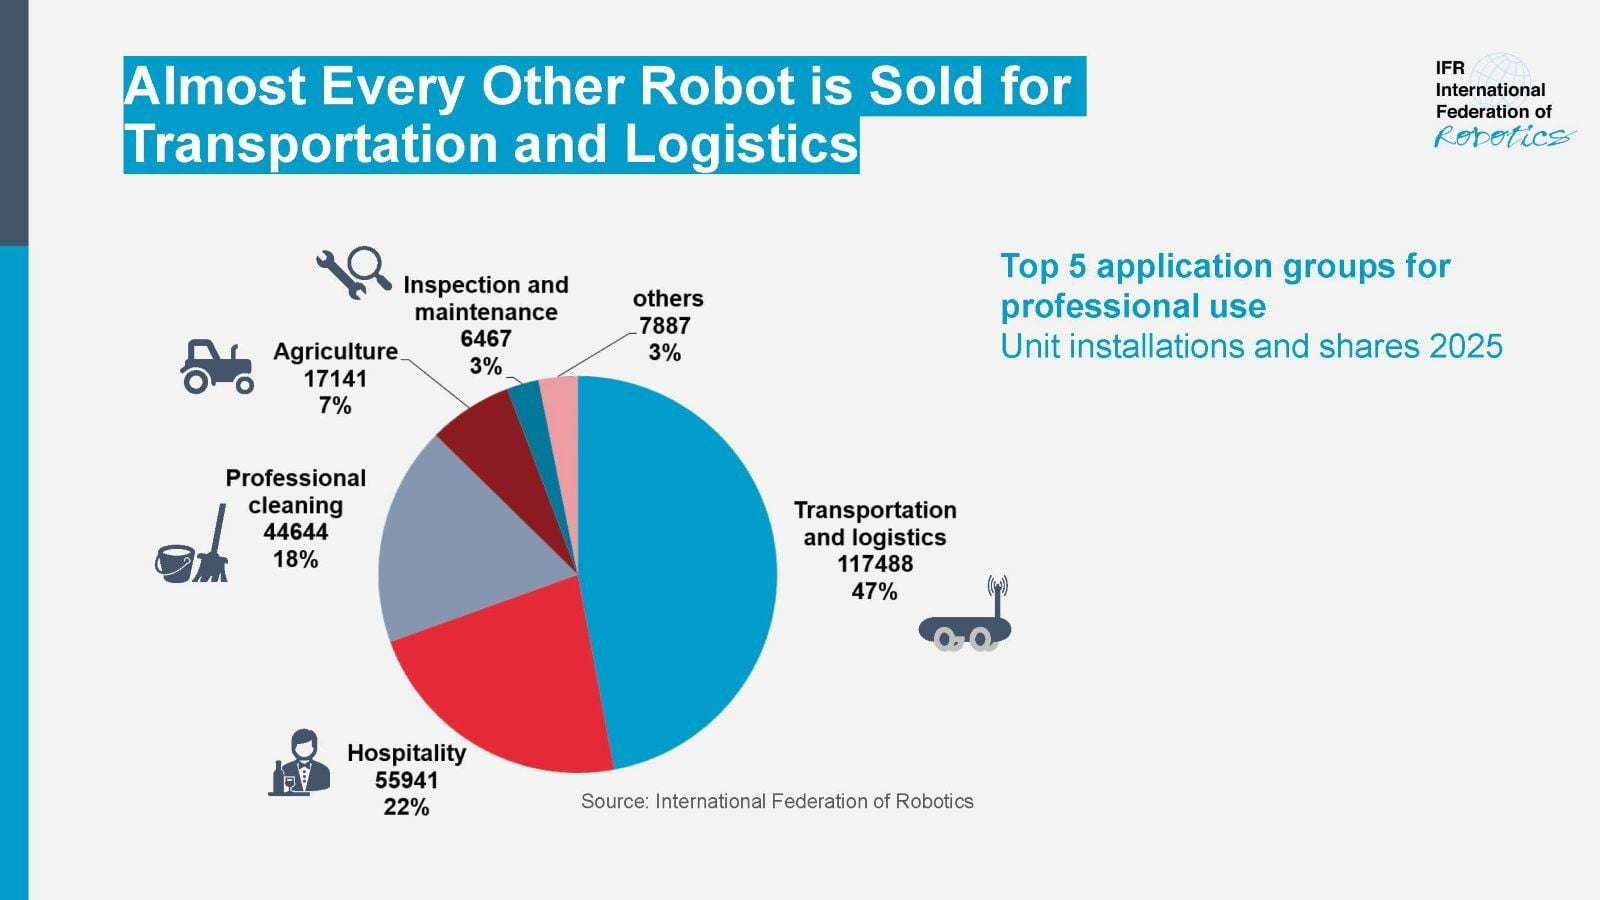
\includegraphics[width=0.95\textwidth]{figsrc/ch01/ifr_service_robots_2025_share.jpg}
    \caption{2025 年專業服務型機器人主要應用類別及銷售占比\cite{ifr2026service}}
    \label{fig:ifr_service_share}
\end{figure}

在技術發展方面，IFR 將人工智慧與自主性、資訊技術與實體控制的整合、人形機器人的可靠性與效率、安全與資安，以及因應人力缺口列為 2026 年的五項重要趨勢，如\cref{fig:ifr_robotics_trends}所示\cite{ifr2026trends}。 其中，自主性、系統整合與安全等方向，與移動操作系統的發展密切相關。對於需要在共享空間中執行任務的機器人，應用需求涉及依據環境資訊調整行動、銜接不同作業階段，以及在運動過程中維持可靠的控制，使感知、規劃與執行能夠相互配合。

\begin{figure}[htbp]
    \centering
    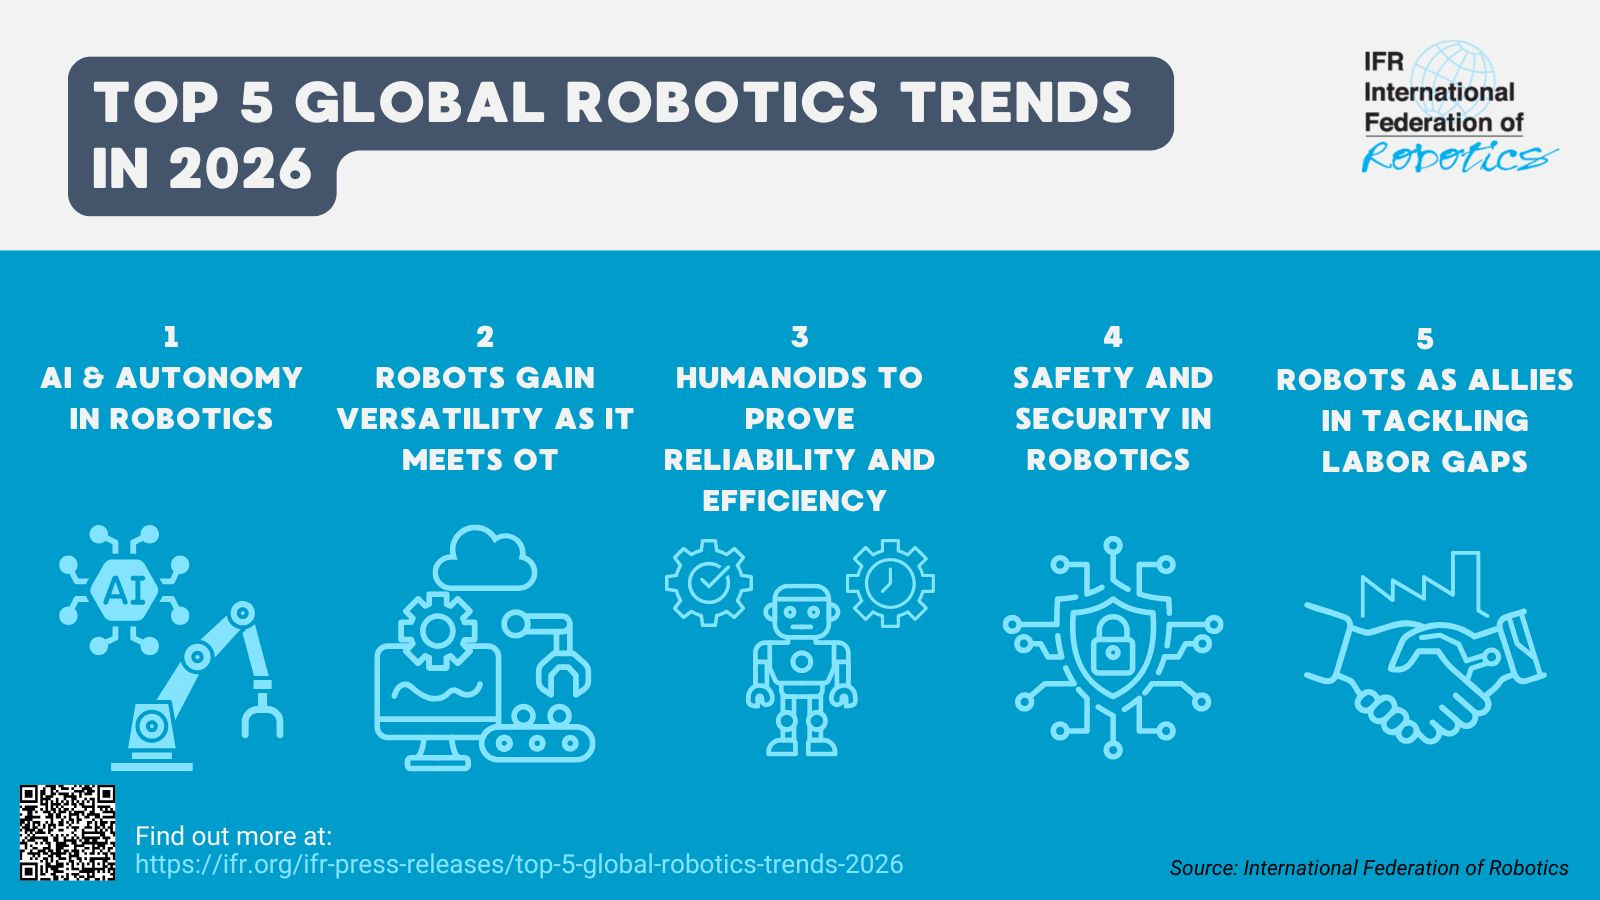
\includegraphics[width=1\textwidth]{figsrc/ch01/ifr_robotics_trends_2026.jpg}
    \caption{2026 年全球機器人產業五項發展趨勢\cite{ifr2026trends}}
    \label{fig:ifr_robotics_trends}
\end{figure}

當任務進一步涉及物件抓取與設備操作時，機器人需要結合移動能力與手臂操作能力。自主移動機械臂（Autonomous Mobile Manipulator Robot, AMMR）整合移動底盤、機械手臂與末端執行器，藉由底盤移動延伸作業範圍，並由手臂完成物件互動，使同一系統能夠在不同位置執行操作任務。IFR 於 2025 年的產業趨勢簡報中，亦將移動機械臂列為因應現場人力與技能短缺的彈性自動化方案之一，強調依工作位置與需求提供支援的應用價值\cite{ifr2025trends}。

在室內服務情境中，一項取物任務可能包含前往指定區域、辨識目標、調整操作位置、抓取與搬運等階段；若行進路徑存在關閉的門扇，或物件位於抽屜內，還需要操作環境中的可動機構。Cen Cheng 等人\cite{cencheng2026safe}將使用者需求、導航、物件辨識、抓取與遞送整合於同一架構，並以實體移動機械臂進行驗證，呈現多項功能銜接的應用需求。 由此可見，移動操作的任務表現受到各階段之間的資訊傳遞與動作接續影響，評估時需要共同考量完整流程的完成情形、操作品質與時間成本。

在動態環境中，底盤運動、手臂操作與目標觀測之間具有相互影響。底盤為避讓障礙而減速或轉向，會改變末端執行器與目標物的相對位置；手臂的可達範圍、關節限制與操作姿態，也會限制底盤可採取的運動。Sun 等人\cite{sun2026motion}針對移動中抓取指出，底盤與手臂的運動耦合，以及感知至執行的延遲，會影響可用的抓取時機。 因此，提升任務效率需要共同安排移動進度與操作時序，並使控制器的預測能夠反映實際命令的執行特性，才能在運動限制下維持追蹤與操作品質。

基於上述產業發展與應用需求，本研究以動態室內環境中的自主移動機械臂為研究對象，探討導航、目標接近與受約束操作之間的協調問題。研究以幾何模型預測控制為基礎，結合環境感知、障礙運動預測與底盤—手臂協同控制，並建立對應命令介面的執行動態模型。透過開門、通行與取物等任務情境，探討兼顧操作品質、動作連續性與任務效率的控制方法。
